% The "%" character denotes a comment
\documentclass[prb,preprint]{revtex4-1}
\usepackage{amsmath}  % needed for \tfrac, \bmatrix, etc.
\usepackage{amsfonts} % needed for bold Greek, Fraktur, and blackboard bold
\usepackage{graphicx} % needed for figures
\usepackage{float}
\usepackage{url}

\begin{document}
\title{Microprocessors - Lab 04: TMP36}
\author{Adam Stammer}
%\email{adam.stammer@go.winona.edu}

\date{\today}

%if you include an abstract, it goes here
\begin{abstract}
The TMP36 temperature sensor is quite common due to it's ease of use and low cost. It isn't immensely accurate, but for many projects it's good enough. In this Lab I set up the TMP36 to report the temperature in degrees celcius using the voltage to temperature algorithm defined in the datasheet. Once that was achieved I used an LED to simulate the automatic controlling of a heater to maintain a particular temperature. From there I added additional output through a 16x2 LCD display.
\end{abstract}

\maketitle
%title page ends here




\section{TMP36}
The basic hookup of the TMP36 can be seen in the figure below. There are numerous tutorials on the internet to aid in this though the datasheet makes it quite clear on its own. I used 3.3V on the Vcc pin just to make sure I didn't burn the sensor out, as I did not have a backup. The GND pin was hooked directly to ground, and the output pin hooked to A1. From A1 we can read a voltage between 0 and 5 volts, though the quantity read ranges from 0 to 1023.

\begin{figure}[H]
	\centering
	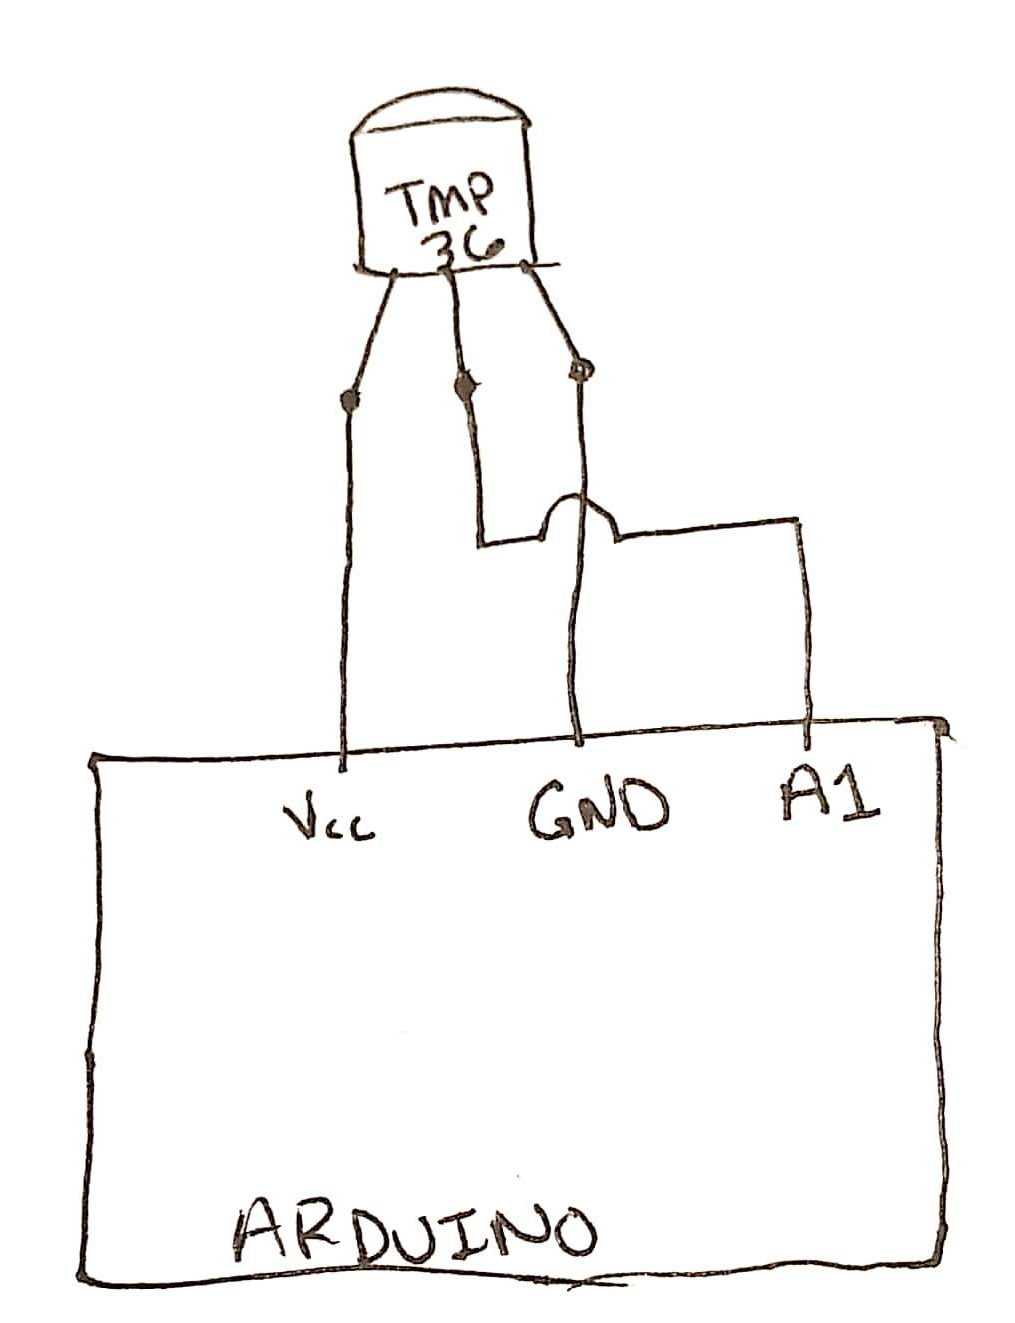
\includegraphics[width=2in]{schem.jpg}
	\caption{TMP36 Wiring}
	\label{fig1}
\end{figure}

Since the measured quantity is not an actual temperature, we need to transform this input curve to another one. The temperature range of the TMP36 varies ever so slightly from one datasheet to the next, but in general it's around -40C-150C, though accuracy drops above 125C. So we need to transform our range of 0-1023 to -40-150. I won't go into too much detail on that, since I've done so in previous lab reports, and because the datasheets and tutorials give us the following equation.

\begin{figure}[H]
	\centering
	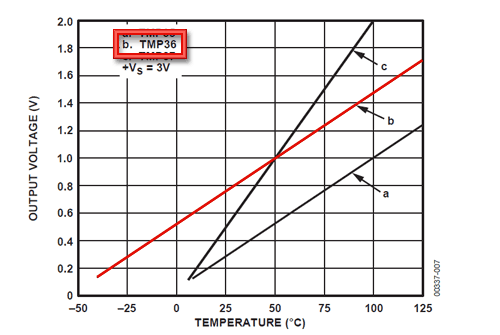
\includegraphics[width=5.75in]{tmp36graph.png}
	\caption{Temperature Transform Graph}
	\label{fig1}
\end{figure}


\begin{equation}
Temperature_{centirgrade} = [(voltage_{mV}) - 500] / 10
\end{equation}

This means we just need to get the input voltage in milliVolts instead of the 0-1023. If we multiply our input reading by 5V, we get our input voltage in Volts. Multiply that by 1000, and we have our input in mV. With this we can rewrite the transform equation as the following.


\begin{equation}
Temperature_{centirgrade} = [([R_{in}/1023] * 5000) - 500] / 10
\end{equation}

Implementing this equation is easy enough, so I won't go into detail in that. The code the should accompany this report will contain what is necessary to do so. To test this, I used the Serial Monitor to print the temperature data back to the PC, from which I graphed the data using Octave. In this test I let the temperature settle at what can be deemed room temperature, then I touched the temperature sensor to heat it up, after which I let it go and watched let it cool back down. As you can see, the sensor was able to heat up much faster than it cooled down.

\begin{figure}[H]
	\centering
	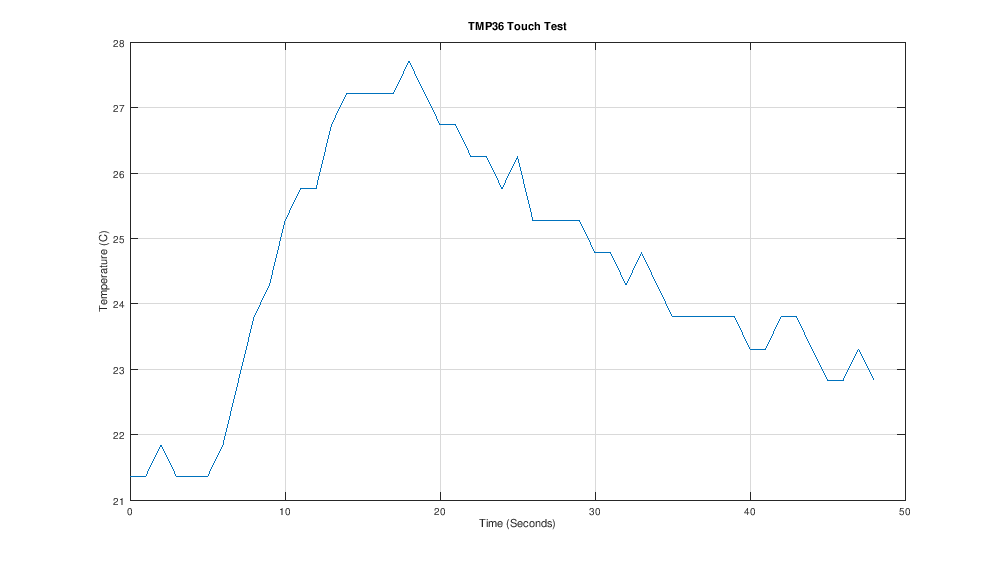
\includegraphics[width=5.75in]{graph.png}
	\caption{TMP36 Measurements}
	\label{fig1}
\end{figure}

\section{Heater}
From here I hooked a "heater" up to A2, but used A2 as a digital output. If it were a real heater, this would much more likely be a relay since the arduino can't handle as much power as a heater would require. Instead of a heater I used a red LED with a resistor to limit current. Adding a simple if/else allows me to toggle A2 on or off based on a temperature conditional. Using the collected data in the graph above I decided that for the sake of testing, a threshold of 25C was adequate. If the temperature is under 25C, turn the heater on, otherwise, turn it off. To see this in action, a video of this project being tested can be found at \url{https://mediaspace.minnstate.edu/media/Heater+TMP36/1_froeko5d}.

\section{LCD}
I still had an LCD screen hooked up from the in class example. The information required to do this can be found on the datasheet of LCD, but I strongly suggest using an online tutorial. The arduino LCD "HelloWorld" example also has all of the information needed.
With that hooked up and displaying a test message, I added commands within the if/else mentioned above to print out a "Heater On"/"Heater Off" message based on what the LED was set to, and also print out the temperature. This can be seen in action at \url{https://mediaspace.minnstate.edu/media/LCD+%2B+TMP36+Heater+Test/1_yc35s2xp}.

\section{Accuracy}
We have to ask ourselves how accurate this setup is. Not just how accurate the sensor itself is, but how effective the implementation is. If we pretend that the TMP36 has perfect accuracy, which of course it doesn't but we're just pretending, we can look at the arduino as the limiting factor. Since the input ranges from 0 to 1023, we just have to look at the output difference from one input to the next. using the same transform equation mentioned at the very beginning, we'll just use 500 and 501 as inputs.

\begin{equation}
23.314 = [([150/1023] * 5000) - 500] / 10
\end{equation}

\begin{equation}
23.803 = [([151/1023] * 5000) - 500] / 10
\end{equation}

Subtracting one from the other gives us a minimum difference of .489C. The TMP36 datasheet says that before it gets above 125C, it is accurate to $\pm$ .5C. That means the accuracy of the device is pretty similar to that of the arduino itself, making neither one much of a limiting factor compared to the other. This is generally considered ideal. Unfortuantely, if the specific accuracy of a TMP36 output is at the minimum, .5C, and the arduino is also at the minimum specific accuracy in the same direction, we end get an overall accuracy of $\pm$1C. It is interesting that there are two best cases here though. If both the sensor and the arduino are at maximum accuracy, we get an accurate answer. The other case, is that one is negatively inaccurate, and the other is positively inaccurate by the same degree. The inaccuracies cancel each other out and we get an accurate answer anyway. Unfortunately, it's very hard to test this kind of thing since any other measuring device used could also be inaccurate.

%\begin{thebibliography}{99}
% The numeral (here 99) in curly braces is nominally the number of entries in
% the bibliography. It's supposed to affect the amount of space around the
% numerical labels, so only the number of digits should matter--and even that
% seems to make no discernible difference.
%Not Requested
%\end{thebibliography}

\end{document}
